%&pdflatex
\documentclass[final,leqno]{siamltex}
%\documentclass[10pt,onecolumn]{article}
\usepackage[top=2cm,bottom=3cm,left=3.5cm,right=3.5cm]{geometry}
\usepackage[utf8]{inputenc}
\usepackage{amsmath,amssymb,amsfonts,mathrsfs}
\let\proof\relax 
\let\endproof\relax
\usepackage{listings}
\usepackage{array}
\usepackage{mathtools}
\usepackage{dsfont}
\usepackage{graphicx}
\usepackage{pdfpages}
\usepackage[textsize=footnotesize,color=green]{todonotes}
\usepackage{algorithm, algorithmic}
\usepackage{array}
\usepackage{bm}
\usepackage{tikz}
\usepackage{subfigure}
\usepackage[normalem]{ulem}

%\usepackage{lineno}
%\pagewiselinenumbers
%\usepackage{uselinenofix}


\newcommand{\bs}[1]{\boldsymbol{#1}}

\newcommand{\equaldef}{\stackrel{\mathrm{def}}{=}}

\newcommand{\tablab}[1]{\label{tab:#1}}
\newcommand{\tabref}[1]{Table~\ref{tab:#1}}

\newcommand{\theolab}[1]{\label{theo:#1}}
\newcommand{\theoref}[1]{\ref{theo:#1}}
\newcommand{\eqnlab}[1]{\label{eq:#1}}
\newcommand{\eqnref}[1]{\eqref{eq:#1}}
\newcommand{\seclab}[1]{\label{sec:#1}}
\newcommand{\secref}[1]{\ref{sec:#1}}
\newcommand{\lemlab}[1]{\label{lem:#1}}
\newcommand{\lemref}[1]{\ref{lem:#1}}

\newcommand{\mb}[1]{\mathbf{#1}}
\newcommand{\mbb}[1]{\mathbb{#1}}
\newcommand{\mc}[1]{\mathcal{#1}}
\newcommand{\nor}[1]{\left\| #1 \right\|}
\newcommand{\snor}[1]{\left| #1 \right|}
\newcommand{\LRp}[1]{\left( #1 \right)}
\newcommand{\LRs}[1]{\left[ #1 \right]}
\newcommand{\LRa}[1]{\left\langle #1 \right\rangle}
\newcommand{\LRc}[1]{\left\{ #1 \right\}}
\newcommand{\LRb}[1]{\left| #1 \right|}

\newcommand{\tanbui}[2]{\textcolor{blue}{\sout{#1}} \textcolor{red}{#2}}
\newcommand{\Grad} {\ensuremath{\nabla}}
\newcommand{\Div} {\ensuremath{\nabla\cdot}}
\newcommand{\Nel} {\ensuremath{{N^\text{el}}}}
\newcommand{\jump}[1] {\ensuremath{\LRs{\!\left[#1\right]\!}}}
\newcommand{\uh}{\widehat{u}}
\newcommand{\fnh}{\widehat{f}_n}
\renewcommand{\L}{L^2\LRp{\Omega}}
\newcommand{\pO}{\partial\Omega}
\newcommand{\Gh}{\Gamma_h}
\newcommand{\Gm}{\Gamma_{-}}
\newcommand{\Gp}{\Gamma_{+}}
\newcommand{\Go}{\Gamma_0}
\newcommand{\Oh}{\Omega_h}

\newcommand{\eval}[2][\right]{\relax
  \ifx#1\right\relax \left.\fi#2#1\rvert}

\def\etal{{\it et al.~}}

\newcommand{\vect}[1]{\ensuremath\boldsymbol{#1}}
\newcommand{\tensor}[1]{\underline{\vect{#1}}}
\newcommand{\del}{\Delta}
\let\grad\relax
\newcommand{\grad}{\nabla}
\newcommand{\curl}{\grad \times}
\renewcommand{\div}{\grad \cdot}
\newcommand{\ip}[1]{\left\langle #1 \right\rangle}
\newcommand{\eip}[1]{a\left( #1 \right)}
\newcommand{\pd}[2]{\frac{\partial#1}{\partial#2}}
\newcommand{\pdd}[2]{\frac{\partial^2#1}{\partial#2^2}}

\newcommand{\circone}{\ding{192}}
\newcommand{\circtwo}{\ding{193}}
\newcommand{\circthree}{\ding{194}}
\newcommand{\circfour}{\ding{195}}
\newcommand{\circfive}{\ding{196}}

\def\arr#1#2#3#4{\left[
\begin{array}{cc}
#1 & #2\\
#3 & #4\\
\end{array}
\right]}
\def\vecttwo#1#2{\left[
\begin{array}{c}
#1\\
#2\\
\end{array}
\right]}
\def\vectthree#1#2#3{\left[
\begin{array}{c}
#1\\
#2\\
#3\\
\end{array}
\right]}
\def\vectfour#1#2#3#4{\left[
\begin{array}{c}
#1\\
#2\\
#3\\
#4\\
\end{array}
\right]}

%\newtheorem{proposition}{Proposition}
%\newtheorem{corollary}{Corollary}
%\newtheorem{theorem}{Theorem}
%\newtheorem{lemma}{Lemma}

\newcommand{\G} {\Gamma}
\newcommand{\Gin} {\Gamma_{in}}
\newcommand{\Gout} {\Gamma_{out}}
\newcommand{\insub}{{\rm in}}
\newcommand{\outsub}{{\rm out}}

\newtheorem{remark}{Remark}

\title{Notes on a nonconforming FEM}
\author{Jesse Chan}
\date{}
\begin{document}

\maketitle

\section{A hybrid nonconforming method}

Consider a coercive variational formulation
\[
a(u,v) = l(v), \quad \forall v\in V.
\]
We assume further that $a(u,v)$ is coercive when restricted to a single element $u,v \in V(K)$.  
Standard methods approximate $u$ using a conforming subspace of $V$.  If we choose instead a broken test space 
\[
V_h \coloneqq \LRc{ v\in \L, \left.v\right|_K \in V(K)},
\]
 we can enforce continuity between elements by penalizing the jumps of $e$ using a Lagrange multiplier method
\begin{align*}
a_h(u,v) + \LRa{\lambda, \jump{v}}_{\Gh}&= l(v)\\
\LRa{\delta \lambda, \jump{u}}_{\Gh} &= 0.
\end{align*}
where $a_h(u,v) = \sum a_K(u,v)$, and  $\lambda$ is a function with support only on $\Gh$, the mesh skeleton. The advantage of this formulation is that the degrees of freedom for $e$ can be condensed out and eliminated, leaving a positive definite system for $\lambda$.  

\section{Stability analysis}

We define norms on our variables $u$ and $\lambda$:
\begin{align*}
\nor{u}_{\Oh}^2 &\coloneqq \sum_{K\in \Oh} a_K(u,u)\\
\nor{\lambda}_{\Gh} &\coloneqq \min_{q\in Q, \gamma_Q(q)_{\Gh} = \lambda} \nor{q}_{Q}.
\end{align*}
where $\lambda$ is discretized as the trace of some space $Q$ with trace $\gamma_Q(q)$, such that $\gamma_Q(q)$ is dual to $\gamma_V(u)$s, the trace of $u$, on $\Gh$. 
We also define an auxiliary norm on the jumps of functions in $V_h$
\[
\nor{\jump{v}}_{\Gh} \coloneqq \sup_{\lambda} \frac{\LRa{\lambda,\jump{v}}_{\Gh}}{\nor{\lambda}_{\Gh}}
\]
Since the condensed system is equivalent to the mixed system, we can use Brezzi mixed theory to analyze the stability of this method.  We require two conditions
\begin{itemize}
\item Inf-sup relating the two spaces
\[
\inf \sup \frac{\LRa{\lambda,\jump{u}}_{\Gh}}{\nor{\lambda}_{\Gh}\nor{u}_{\Oh}}  \geq \gamma_0 > 0,
\]
\item Inf-sup in the kernel: for $u_0 \in U_0\coloneqq \LRc{u\in V: \LRa{\lambda,\jump{u}}_{\Gh} = 0}$
\[
\inf \sup \frac{a_h(u_0,v)}{\nor{u_0}_{\Oh}\nor{v}_{\Oh}} \geq \gamma_0 > 0,
\]
\end{itemize}
The second condition holds trivially due to coercivity of $a_h(u,v)$ on $K$, while the first condition reduces to 
\[
\nor{\jump{u}}_{\Gh} \geq \gamma_0\nor{u}_{\Oh}.
\]
In other words, the jumps of $u$ should be bounded from below by the nonconforming broken norm.  

\subsection{Example: Poisson's equation with first order term} 

We consider the equation with $\alpha > 0$
\[
-\Delta u + \alpha u = f
\]
which gives the following conforming variational formulation
\[
a(u,v) \coloneqq \LRp{\grad u,\grad v}_{\Omega} + \alpha\LRp{u,v}_{\Omega} = \LRp{f,v}_{\Omega}.
\]
The nonconforming formulation is given by 
\[
a_h(u,\lambda,v) \coloneqq \sum_{K \in \Oh}\LRs{ a_K(u,v) + \LRa{\lambda,v}_{\partial K}} = \sum_{K \in \Oh} a_K(u,v) + \LRa{\lambda,\jump{v}}_{\Gh}
\]
In this specific case, $\lambda$ is the trace of Raviart-Thomas elements, with corresponding norm
\[
\nor{\lambda}_{\Gh} \coloneqq \min_{q\in H({\rm div}), \left.q\cdot n\right|_{\Gh} = \lambda} \nor{q}_{H({\rm div})}.
\]
The first condition then requires only a mesh-independent Poincare inequality for broken $H^1$ functions, given in Lemma 4.2 of \cite{analysisDPG}.  
\begin{align*}
\nor{v}_{\Oh} &\leq C\LRp{\nor{\grad v}_{\Oh} + \nor{\jump{v}}_{\Gh}}
\end{align*}

Both the primal and original $C_0$ mixed DPG methods for convection-diffusion display optimal rates, and display nearly identical $L^2$ errors on the same mesh.  Below are comparisons of $L^2$-errors under uniform refinement.  The flux variable $\lambda$ is taken to be the trace of Raviart-Thomas elements of equal order to the field variables $u$ (which gives a polynomial degree of $p-1$ on the edge).  If we decrease our polynomial degree to be Raviart-Thomas elements of order $p-1$ instead of $p$, the rate of convergence falls to $h^p$ for $L^2$ errors.\footnote{In general, the optimal rate of convergence appears to be limited to $p_f+1$.}
%
%%p =1
%conf_rates =  [1.8345732590626442, 1.956593598614242, 1.9889774729025818]
%nconf_rates =  [1.9689541205877867, 1.9972377274555484, 2.0011447175440362]
%%p = 2
%conf_rates =  [3.0722694270062911, 3.0240457527815638, 3.0063546464093531]
%nconf_rates =  [3.1470283208817555, 3.0526826535868672, 3.0168130426196647]
%%p = 3
%conf_rates =  [4.0178487745609379, 4.0201684559295625, 4.0124170028446269]
%nconf_rates =  [3.9969917961533792, 4.0119390965563149, 4.0088579511366031]

\begin{figure}
\centering
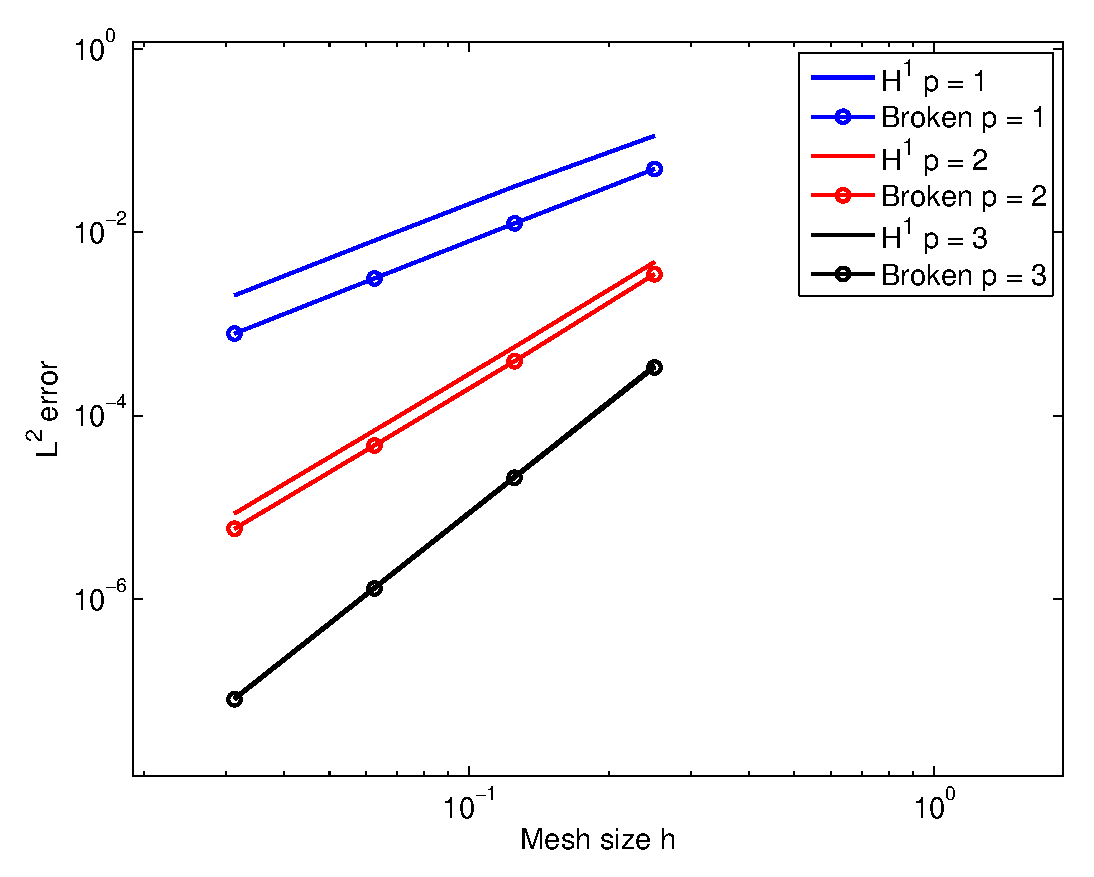
\includegraphics[width=.6\textwidth]{figs/poisson_rates.eps}
  \caption{$L^2$ errors for conforming vs nonconforming discretizations.}
\end{figure}

\begin{figure}
\centering
\subfigure[$p_f = p$]{
  \begin{tabular}{| l || c | r |}
   \hline
    Order & Conforming & Non-conforming\\
    \hline
    $p=1$ & 1.98898 & 2.00114 \\ \hline
    $p=2$ & 3.00635 & 3.01681 \\ \hline
    $p=3$ & 4.01242 & 4.00886 \\
    \hline
  \end{tabular}
  }
  \subfigure[$p_f = p-1$]{
  \begin{tabular}{| l || c |}
   \hline
    Order & Non-conforming\\
    \hline
    $p=1$ & N/A  \\ \hline
    $p=2$ & 2.00317  \\ \hline
    $p=3$ & 2.98382 \\
    \hline
  \end{tabular}
  }
  \caption{Rates of convergence for conforming vs nonconforming discretizations.}
\end{figure}

%The first condition for stability holds if we use two modifications of two lemmas for locally harmonic functions (i.e. minimum energy extensions of functions supported on the mesh skeleton) from \cite{analysisDPG}
%\cite{primalDPG}: 
%\begin{align*}
%\nor{v}_{\Oh} &\leq C\LRp{\nor{P \grad v}_{\Oh} + \nor{\jump{v}}_{\Gh}}\\
%\nor{\grad v}_{\Oh} &\leq \nor{P \grad v}_{\Oh} + C\nor{\jump{v}}_{\Gh}
%\end{align*}

%\section{Nonconformity analysis}
%
%Brenner's theory on nonconforming finite element methods - estimation of consistency error 
%\[
%\nor{u-u_h}_{V_h} \leq C\LRp{\inf_{v\in V_h} \nor{u-v}_{V_h} + \sup_{w\in V_h}\frac{a_h(u-u_h,w)}{\nor{w}_{V_h}}}
%\]
%Can we somehow use this to show 

%\section{Initial numerical results}


\bibliographystyle{unsrt}
\bibliography{paper}

\end{document}
